%%%%%%%%%%%%%%%%%%%%%%%%%%%%%%%%%%%%%%%%%
% Beamer Presentation
% LaTeX Template
% Version 1.0 (10/11/12)
%
% This template has been downloaded from:
% http://www.LaTeXTemplates.com
%
% License:
% CC BY-NC-SA 3.0 (http://creativecommons.org/licenses/by-nc-sa/3.0/)
%
%%%%%%%%%%%%%%%%%%%%%%%%%%%%%%%%%%%%%%%%%

%----------------------------------------------------------------------------------------
%	PACKAGES AND THEMES
%----------------------------------------------------------------------------------------

\documentclass{beamer}
\AtBeginSection[]
{
  \begin{frame}
    \frametitle{Table of Contents}
    \tableofcontents[currentsection]
  \end{frame}
}
\newenvironment<>{varblock}[2][.9\textwidth]{%
  \setlength{\textwidth}{#1}
  \begin{actionenv}#3%
    \def\insertblocktitle{#2}%
    \par%
    \usebeamertemplate{block begin}}
  {\par%
    \usebeamertemplate{block end}%
  \end{actionenv}}
  
\mode<presentation> {

% The Beamer class comes with a number of default slide themes
% which change the colors and layouts of slides. Below this is a list
% of all the themes, uncomment each in turn to see what they look like.

%\usetheme{default}
%\usetheme{AnnArbor}
%\usetheme{Antibes}
%\usetheme{Bergen}
%\usetheme{Berkeley}
%\usetheme{Berlin}
%\usetheme{Boadilla}
%\usetheme{CambridgeUS}
%\usetheme{Copenhagen}
%\usetheme{Darmstadt}
%\usetheme{Dresden}
%\usetheme{Frankfurt}
%\usetheme{Goettingen}
%\usetheme{Hannover}
%\usetheme{Ilmenau}
%\usetheme{JuanLesPins}
%\usetheme{Luebeck}
\usetheme{Madrid}
%\usetheme{Malmoe}
%\usetheme{Marburg}
%\usetheme{Montpellier}
%\usetheme{PaloAlto}
%\usetheme{Pittsburgh}
%\usetheme{Rochester}
%\usetheme{Singapore}
%\usetheme{Szeged}
%\usetheme{Warsaw}

% As well as themes, the Beamer class has a number of color themes
% for any slide theme. Uncomment each of these in turn to see how it
% changes the colors of your current slide theme.

%\usecolortheme{albatross}
%\usecolortheme{beaver}
%\usecolortheme{beetle}
%\usecolortheme{crane}
%\usecolortheme{dolphin}
%\usecolortheme{dove}
%\usecolortheme{fly}
%\usecolortheme{lily}
%\usecolortheme{orchid}
%\usecolortheme{rose}
%\usecolortheme{seagull}
%\usecolortheme{seahorse}
%\usecolortheme{whale}
%\usecolortheme{wolverine}

%\setbeamertemplate{footline} % To remove the footer line in all slides uncomment this line
%\setbeamertemplate{footline}[page number] % To replace the footer line in all slides with a simple slide count uncomment this line

%\setbeamertemplate{navigation symbols}{} % To remove the navigation symbols from the bottom of all slides uncomment this line
}

\usepackage{graphicx} % Allows including images
\usepackage{booktabs} % Allows the use of \toprule, \midrule and \bottomrule in tables
\usepackage{verbatim}
\usepackage{minted}
\usepackage{xcolor}
\usepackage{color}

\usepackage{listings}% http://ctan.org/pkg/listings
\usepackage{xcolor}% http://ctan.org/pkg/xcolor
\definecolor{bluekeywords}{rgb}{0.13,0.13,1}
\definecolor{greencomments}{rgb}{0,0.5,0}
\definecolor{turqusnumbers}{rgb}{0.17,0.57,0.69}
\definecolor{redstrings}{rgb}{0.5,0,0}


\lstdefinelanguage{FSharp}
    {morekeywords={let, new, match, with, rec, open, module, namespace, type, of, member, and, for, in, do, begin, end, fun, function, try, mutable, if, then, else},
    keywordstyle=\color{bluekeywords},
    sensitive=false,
    morecomment=[l][\color{greencomments}]{///},
    morecomment=[l][\color{greencomments}]{//},
    morecomment=[s][\color{greencomments}]{{(*}{*)}},
    morestring=[b]",
    stringstyle=\color{redstrings}
    }

\lstnewenvironment{fslisting}
  {
    \lstset{
        language=FSharp,
        basicstyle=\ttfamily,
        breaklines=true,
        columns=fullflexible}
  }
  {
  }

%----------------------------------------------------------------------------------------
%	TITLE PAGE
%----------------------------------------------------------------------------------------

\title[Functional prototyping]{Functional thinking, a \textbf{universal} tool for the digital world } % The short title appears at the bottom of every slide, the full title is only on the title page

\author{Nicolas Rolland} % Your name
\institute[] % Your institution as it will appear on the bottom of every slide, may be shorthand to save space
{
\medskip
}
\date{\today} % Date, can be changed to a custom date

\begin{document}



\begin{frame}
\titlepage % Print the title page as the first slide
\end{frame}

\begin{frame}
\frametitle{Table of Contents} % Table of contents slide, comment this block out to remove it
\tableofcontents % Throughout your presentation, if you choose to use \section{} and \subsection{} commands, these will automatically be printed on this slide as an overview of your presentation
\end{frame}

%----------------------------------------------------------------------------------------
%	PRESENTATION SLIDES
%----------------------------------------------------------------------------------------

%------------------------------------------------
\section{Types} % Sections can be created in order to organize your presentation into discrete blocks, all sections and subsections are automatically printed in the table of contents as an overview of the talk
%------------------------------------------------

\subsection{why types ?}

\begin{frame}
\frametitle{Types}
\begin{itemize}
\item What is a type ?
\pause
\begin{center}
\begin{minipage}{5cm}
\begin{varblock}[4cm]{Type}
A type is a set of values.
\end{varblock}
\end{minipage}
\end{center}
\pause
\end{itemize}
why do we need to think of it in typed functional programming ? 
\begin{itemize}
\item a value is a value  e.g. $1$
\pause
\item a \textbf{function} is a value too ! 
\inputminted[fontsize=\scriptsize]{fsharp}{00-functionasvalue.fs}
\pause
\item hence everything is a value, \textbf{everything} has a type !
\end{itemize}

\end{frame}
\begin{frame}
\frametitle{Using types}
\begin{itemize}
\pause
\item by restriction we get correctness - The computer tells us the errors
\pause
\item restriction tells readers a specification - We can communicate to other people
\end{itemize}
\pause
\begin{itemize}
\item Types should be helping you, not get in your way.
\item  \textbf{No need to write} the types in F\#. Less work AND more security !
\item You can write the types for the purpose of communication with others
\end{itemize}
\end{frame}

\begin{frame}
\frametitle{Warm-up exercices }
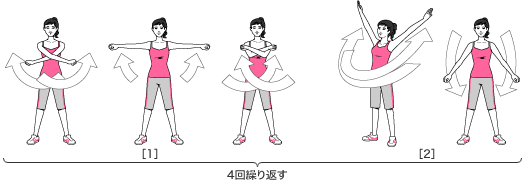
\includegraphics[height=5cm,width=12cm]{image002.png}
\end{frame}

\subsection{Warm-up exercices}

\begin{frame}
\frametitle{what can I do with a value of this type ?}
\begin{center}
\begin{minipage}{5cm}
\begin{varblock}[4cm]{Type1}
$$\left( \right) \longrightarrow T$$
\end{varblock}
\end{minipage}
\end{center}
\pause
\inputminted{fsharp}{10-delayexample.fs}

\pause
lazy values !
\pause
\inputminted{fsharp}{11-delayexample.fs}

$$  T  \cong  \left( \right)  \rightarrow T   $$

\begin{columns}[c] % The "c" option specifies centered vertical alignment while the "t" option is used for top vertical alignment
\pause


\column{.45\textwidth} % Left column and width
\begin{align*}
\mbox {let  delay  x} &= fun \left( \right) \rightarrow x  &&: T  \rightarrow \left( \left( \right)  \rightarrow T \right)   \\
\mbox {let  force  f} &= f   \left( \right)   &&: \left( \left( \right)  \rightarrow T \right)  \rightarrow T      
\end{align*}
\column{.5\textwidth} % Right column and width
\begin{eqnarray*}
\mbox{delay force } &&=  Id_{  \left( \right)  \rightarrow T  } \\
\mbox{force delay } &&= Id_{  T } 
\end{eqnarray*}
\end{columns}


\end{frame}


\begin{frame}
\frametitle{what can I do with a value of this type ?}
\begin{center}
\begin{minipage}{5cm}
\begin{varblock}[10cm]{Type2}

\begin{eqnarray*}
\mbox {type Type2}<T> = && \vert\,  \mbox{Case1 of }  \left(  T * Type2<T> \right)    \\
									 && \vert \, \mbox{Case0  }       
\end{eqnarray*}

\end{varblock}
\end{minipage}
\end{center}
\pause
\inputminted{fsharp}{13-listexample.fs}
\pause
This is a list !
\inputminted{fsharp}{14-listexampleUse.fs}


\end{frame}


\begin{frame}
\frametitle{what can I do with a value of this type ?}
\begin{center}
\begin{minipage}{5cm}
\begin{varblock}[10cm]{Type3}

\begin{eqnarray*}
\mbox {type RComp}<T> = && \vert\,  \mbox{NotYet of }  \left(  \left( \right)  \rightarrow RComp<T> \right)    \\
									 && \vert \, \mbox{Finished  of } T       
\end{eqnarray*}

\end{varblock}
\end{minipage}
\end{center}
\pause
\inputminted{fsharp}{15-resumableExample.fs}
\pause
Resumable computation !


\end{frame}

\subsection{IEnumerable and IObservable} % types make it readable and simple


\begin{frame}
\frametitle{can you recognize IEnumerable ?}
What is a value of type IEnumerable ?
\pause
 a sequence of items

\pause
\begin{center}
\begin{minipage}{5cm}
\begin{varblock}[10cm]{Item}
\begin{align*}
&\mbox{type Item of } T  &&= 		 \vert\, \mbox{Finished }   \vert\, \mbox{Value of } T 		 				\end{align*}
\end{varblock}
\end{minipage}
\end{center}
\pause
\begin{center}
\begin{minipage}{5cm}
\begin{varblock}[10cm]{IEnumerable}
\begin{align*}
&\mbox {type IEnumerable}<T> &&=  	\left( \right)  \rightarrow \left(\left( \right) \rightarrow \mbox{Item of } T   \right)     
\end{align*}
\end{varblock}
\end{minipage}
\end{center}
\end{frame}

\begin{frame}
\frametitle{Object Oriented way}
%from http://referencesource.microsoft.com/
\begin{columns}[c] % The "c" option specifies centered vertical alignment while the "t" option is used for top vertical alignment
\pause


\column{.45\textwidth} % Left column and width
\inputminted{csharp}{01-IEnumerable.cs}
\column{.5\textwidth} % Right column and width
\begin{itemize}
\item How can I read the protocol ?
\item Should I call MoveNext first ?
\item What is the value of current after enumeration is finished ?
\item How can I make sure current is not used after enumeration is finished ?
\end{itemize}
\end{columns}
\end{frame}

\begin{frame}
\begin{center}
\begin{minipage}{5cm}
\begin{varblock}[10cm]{IObservable / Reactive}
\begin{align*}
&\mbox {type IObservable}<T> &&=  \left(\mbox{Item of } T \rightarrow \left( \right)   \right)  \rightarrow  	\left( \right)    
\end{align*}
\end{varblock}
\end{minipage}
\end{center}
\begin{center}
\begin{minipage}{5cm}

\pause
\begin{varblock}[10cm]{IEnumerable}
\begin{align*}
&\mbox {type IEnumerable}<T> &&=  	\left( \right)  \rightarrow \left(\left( \right) \rightarrow \mbox{Item of } T   \right)   
\end{align*}
\end{varblock}
\end{minipage}
\end{center}
\begin{itemize}
\item Don't they look similar .... ? 
\pause
\item why ?
\end{itemize}
\end{frame}




\begin{frame}
\frametitle{What is a type - take 2}
\begin{itemize}
\item What is a type and why do we need to think of it ?
\pause
\begin{center}
\begin{minipage}{8cm}
\begin{varblock}[8cm]{Type}
A type is a \textbf{computable specification}
\end{varblock}
\end{minipage}
\end{center}
\pause
\end{itemize}
\begin{itemize}
\item Domain Driven Design : the architecture \textbf{is} the code
\end{itemize}
\end{frame}


\begin{frame}
\frametitle{Together }
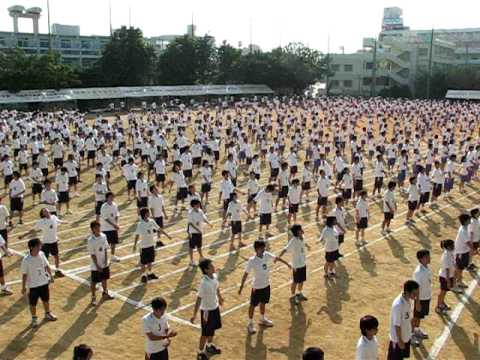
\includegraphics[height=8cm,width=12cm]{hqdefault.jpg}
\end{frame}

\section{ Universals, programming against the interface and existentials}

\subsection{universals }
\begin{frame}[fragile]
\frametitle{Universals}
\begin{center}
\begin{minipage}{9cm}
\begin{varblock}[9cm]{Type}
\inputminted[fontsize=\scriptsize]{fsharp}{03-universal.fs}
\end{varblock}
\end{minipage}
\end{center}
\begin{itemize}
\item What is the type of  $Empty $ \pause   ? $$Empty : \forall T . \, List<T> $$
\item What is the type of  $Cons $ \pause   ? $$Cons : \forall T . \, T* List<T> \rightarrow List<T> $$

\end{itemize}
\end{frame}

\begin{frame}[fragile]
\begin{itemize}
\frametitle{Universals}
\item What is the type of  $Empty $  ? $Empty : \forall T . \, List<T> $
\item "I don't need to know anything about the type to do my job, \textbf{I} will only refer to it \textbf{opaquely} as T"

\begin{minipage}[t]{0.48\linewidth}
\begin{varblock}[5cm]{ implementer of $List<T>$}
does not know $T$
\end{varblock}
\end{minipage}
\hfill%
\begin{minipage}[t]{0.48\linewidth}
\begin{varblock}[5cm]{ user of $List<T>$}
provide the type T
\end{varblock}
\end{minipage}
\end{itemize}
\end{frame}

\subsection{it sounds like "L" in SOLID .. } 

\begin{frame}
\inputminted[mathescape,
                     numbersep=5pt,
                     fontsize=\scriptsize]{fsharp}{02-liskov.fs}
\frametitle{Liskov substitution "principle" - Program to interface}

\end{frame}



\subsection{existentials} 


\begin{frame}[fragile]
\frametitle{Existentials}
\begin{itemize} 
\item \textbf{Interfaces} allows to abstract in object oriented programming
\item Like \textbf{universals} types, it "hides" something, but what is the relation  ?
\pause
\item Functional is Mathematics ! Abstraction in FP \textbf{has} to have a precise definition related to universals ! 
\pause
\item Universals definition
  $$empty : \forall T . \,\left( \right) \rightarrow List<T> $$
   suggests "existentials" 
  \begin{align*}
	  absStack : \exists T \{ &empty :\left( \right)\rightarrow T   \\
	  									  &push : int*T \rightarrow T \\
	  									  &pop  : T \rightarrow T \\
  	  									  &top :  T \rightarrow int  \}
  \end{align*}
 \item " I'll use whatever type I want here; you wont know anything about the type, so \textbf{you} can only refer to it \textbf{opaquely} as X"
\end{itemize}
\end{frame}

\begin{frame}
\begin{align*}
	  absStack : \exists T \{ &empty :\left( \right)\rightarrow T   \\
	  									  &push : int*T \rightarrow T \\
	  									  &pop  : T \rightarrow T \\
  	  									  &top :  T \rightarrow int  \}
  \end{align*}
  
 \begin{minipage}[t]{0.5\linewidth}
\begin{varblock}[5.1cm]{ implementer}
Know about the specific type $T$     
\end{varblock}
\end{minipage}
\hfill%
\begin{minipage}[t]{0.48\linewidth}
\begin{varblock}[6cm]{ user}
does not know about the specific type T, only about the interface
\end{varblock}
\end{minipage}
\end{frame}  

\begin{frame}
\frametitle{duality}
\begin{columns}[c] % The "c" option specifies centered vertical alignment while the "t" option is used for top vertical alignment
\pause


\column{.45\textwidth} % Left column and width
\begin{itemize}
\item IEnumerable vs IObservable
\item Universals vs Existentials
\end{itemize}
\column{.5\textwidth} % Right column and width
are examples of applying \textbf{duality}
\end{columns}
\end{frame}



\begin{frame}
\frametitle{Erik Meijer -  he will reverse all your arrows }
\begin{center}
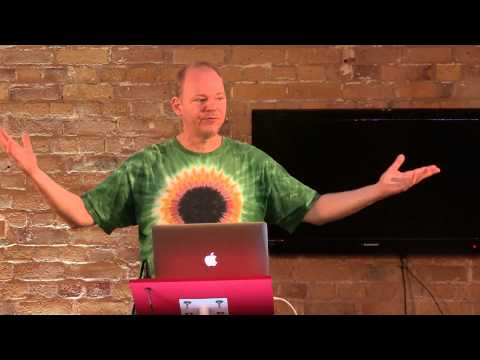
\includegraphics[height=8cm,width=10cm]{0.jpg}
\end{center}
\end{frame}

\begin{frame}
\frametitle{Functional programming and duality 
is old : we know it works }
\begin{center}
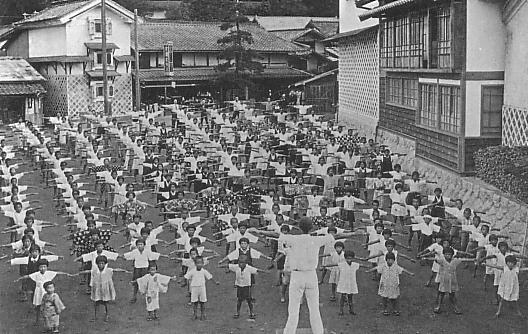
\includegraphics[height=8cm,width=10cm]{Radio_calisthenics_in_1930s.jpg}
\end{center}
\end{frame}

\begin{frame}
\frametitle{encoding in Fsharp}
\inputminted[mathescape,fontsize=\footnotesize]{fsharp}{04-existentials.fs}
\end{frame}


\begin{frame}
\frametitle{stack demo}
\end{frame}

\begin{frame}
\frametitle{Existentials - References}
\footnotesize{
\begin{thebibliography}{99} % Beamer does not support BibTeX so references must be inserted manually as below
\bibitem[Cardelli, 1987]{cw1} Luca Cardelli, Peter Wegner (1985)
\newblock On Understanding Types, Data Abstraction, and Polymorphism
\bibitem[Cook, 2004?]{cook1} William Cook (2009)
\newblock On Understanding Data Abstraction, Revisited
\end{thebibliography}
}
\end{frame}
\section{Prototyping the functional way}

% value computing versus place computing - thinking about the problem, not the technicalities
% when we mutate things, we are doing place.
%  this is where i store my result (mutable) 
%    VS this is what I think my result is at this point in time (immutable)
%  semantic shift with a big impact : immutable is always true, serialazible, sharable.
%                                     most importantly represent only the problem.
% an important step is what value we compute
% One can compute probability distribution //type
% One can compute a parser //what is the type ?

\subsection{Parser combinator}

\begin{frame}
\frametitle{How do we go from here to there ?}

\begin{minipage}[t]{0.48\linewidth}
\begin{varblock}[5cm]{ string}
"[a number is like 1234 but can also be 9.12 ]"
\end{varblock}
\end{minipage}
\hfill%
\begin{minipage}[t]{0.48\linewidth}
\begin{varblock}[6cm]{ value }
\inputminted[mathescape,numbersep=5pt,fontsize=\footnotesize]{fsharp}{08-parsedvalue.fs}
\end{varblock}
\end{minipage}
\pause

This is a job for .....
\pause
grep ?
\pause
imperative ?
\pause
or...
\pause
\resizebox{1.75cm}{!}{$\lambda$ !} 

\end{frame}

\begin{frame}
\frametitle{ lambda man ! }
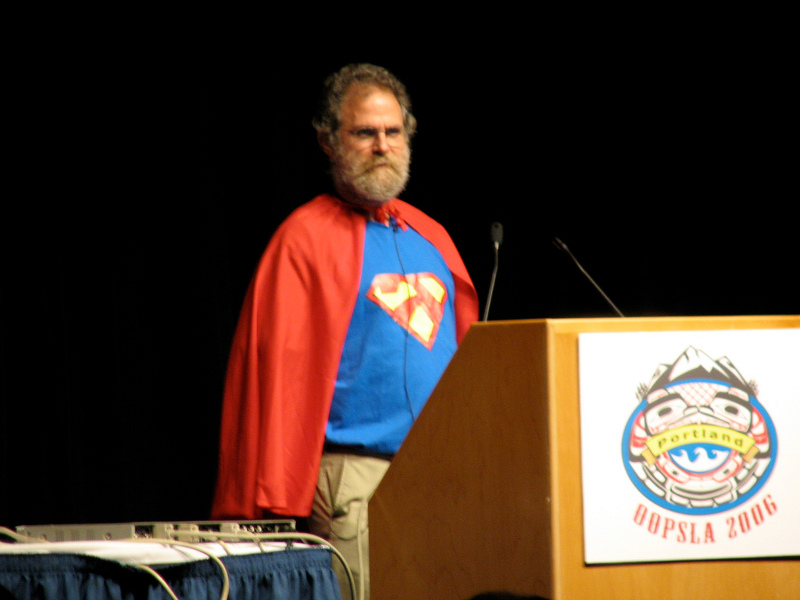
\includegraphics[height=8cm,width=12cm]{lambda-man.jpg}
\end{frame}

\begin{frame}
\frametitle{start with the types}
\pause
\begin{minipage}[t]{0.48\linewidth}
\begin{varblock}{value type}
\inputminted[mathescape,numbersep=5pt,fontsize=\footnotesize]{fsharp}{07-parservalue.fs}
\end{varblock}
\end{minipage}
\hfill%
\begin{minipage}[t]{0.52\linewidth}
\begin{varblock}{ value}
\inputminted[mathescape,numbersep=5pt,fontsize=\footnotesize]{fsharp}{08-parsedvalue.fs}
\end{varblock}
\end{minipage}

\end{frame}
\begin{frame}
\begin{varblock}[10cm]{ parser return type - first try}
\inputminted[mathescape,numbersep=5pt,fontsize=\footnotesize]{fsharp}{06-parsectype.fs}
\end{varblock}

\pause

\begin{varblock}{ reading the parser type}

\begin{itemize} 
\item a parser takes a list of token  in
\item it returns a ParserReturn , and the tokens not yet processed
\pause
\item a ParserReturn is the value represented by the token consumed 
\end{itemize}
\end{varblock}

Ok, but........ "9.12 " : 
\begin{itemize}
\item 9 is a number.. but if we recognize "9" as 9 only, what do we do for ".12" ?
\item $\implies $ the result of a parser depends also on the rest of the string
\end{itemize}
If it matters, it should be part of the returned type of a parser  !
\end{frame}
\begin{frame}
\begin{varblock}[10cm]{ parser return type}
\inputminted[mathescape,numbersep=5pt,fontsize=\footnotesize]{fsharp}{06-parsectypecomplete.fs}
\end{varblock}
e.g. "9.12 " 
\begin{varblock}{ reading the parser type}

\begin{itemize} 
\item Each success contains a recognized value \textbf{along with} the "rest"
\item Because the notion of what is the "rest" is \textbf{dependent} on the $Val$ produced
\item $ParseReturn$ now contains a coherent and actionable unit of information
\end{itemize}
\end{varblock}
\end{frame}

\begin{frame}
\frametitle{demo time}
\end{frame}
\begin{frame}
\frametitle{There are many more tricks to practice}
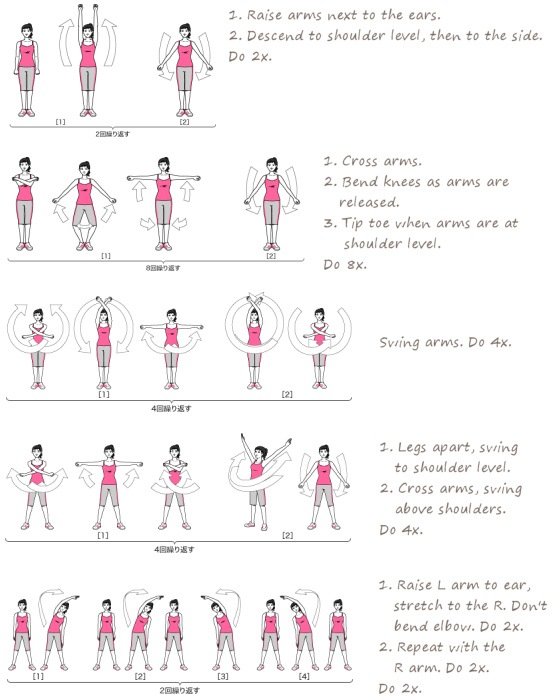
\includegraphics[height=8cm,width=10cm]{radiotaiso1a.jpg}
\end{frame}

\begin{frame}
\Huge{\centerline{The End}}
\end{frame}

%----------------------------------------------------------------------------------------

\end{document}
